%ln8
%cp8m
%cp8t
%cp8r
%ps7

\hyperdef{number}{theory}{\chapter{Number Theory}}\label{number_theory_chap}
\term{Number theory} is the study of the integers.  \emph{Why} anyone
would want to study the integers is not immediately obvious.  First of
all, what's to know?  There's 0, there's 1, 2, 3, and so on, and, oh yeah,
-1, -2, \dots.  Which one don't you understand?  Second, what practical
value is there in it?
%Number theory is
%right at the core of mathematics; even Ug the Caveman surely had some
%grasp of the integers--- at least the positive ones.  In fact, the
%integers are so elementary that one might ask, ``What's to study?''
%There's 0, there's 1, 2, 3 and so on, and there's the negatives.
%Which one don't you understand?  
%Doesn't math become easy when we
%don't have to worry about nasty numbers like $\sqrt{7}$, $1 / \pi$,
%and $i$?  We can even forget about fractions!
The mathematician G. H. \idx{Hardy} expressed pleasure in its
impracticality when he wrote:
%
 \begin{quotation}
 \noindent [Number theorists] may be justified in rejoicing that there
 is one science, at any rate, and that their own, whose very remoteness
 from ordinary human activities should keep it gentle and clean.
 \end{quotation}
%

 Hardy was specially concerned that number theory not be used in
 warfare; he was a pacifist.  You may applaud his sentiments, but he
 got it wrong: Number Theory underlies modern cryptography, which is
 what makes secure online communication possible.  Secure
 communication is of course crucial in war ---which may leave poor
 Hardy spinning in his grave.  It's also central to online commerce.
 Every time you buy a book from Amazon, check your grades on WebSIS,
 or use a PayPal account, you are relying on number theoretic
 algorithms.

%% Divisibility %%%%%%%%%%%%%%%%%%%%%%%%%%%%%%%%%%%%%%%%%%%%%%%%%%%%%%%%%%%%%%%
\section{Divisibility}\label{divisibility_sec}

Since we'll be focussing on properties of the integers, we'll adopt
the default convention in this chapter that \emph{variables range over
integers}, $\integers$.

The nature of number theory emerges as soon as we consider the
\term{divides} relation
\[
a \text{ divides } b \qiff ak = b \text{ for some } k.
\]
The notation, $a$ \index{$\divides$ (divides relation)}$\divides$ $b$, is
an abbreviation for ``$a$ divides $b$.''  If $a \divides b$, then we also
say that $b$ is a \term{multiple} of $a$.  As we've seen, a consequence of
this definition is that every number divides zero.

This seems simple enough, but let's play with this definition.  The
Pythagoreans, an ancient sect of mathematical mystics, said that a number
is \index{perfect number}\term*{perfect} if it equals the sum of its
positive integral divisors, excluding itself.  For example, $6 = 1 + 2 +
3$ and $28 = 1 + 2 + 4 + 7 + 14$ are perfect numbers.  On the other hand,
10 is not perfect because $1 + 2 + 5 = 8$, and 12 is not perfect because
$1 + 2 + 3 + 4 + 6 = 16$.  \idx{Euclid} characterized all the \emph{even}
perfect numbers around 300 BC.  But is there an \emph{odd} perfect number?
More than two thousand years later, we still don't know!  All numbers up
to about $10^{300}$ have been ruled out, but no one has proved that there
isn't an odd perfect number waiting just over the horizon.

So a half-page into number theory, we've strayed past the outer limits of
human knowledge!  This is pretty typical; number theory is full of
questions that are easy to pose, but incredibly difficult to answer.
Interestingly, computer scientists have found ways to turn these
difficulties to their advantage.

\emph{Don't Panic} ---we're going to stick to some relatively benign parts
of number theory.  We rarely put any of these super-hard unsolved problems
on exams :-)

\subsection{Facts About Divisibility}

The lemma below states some basic facts about divisibility that are
\emph{not} difficult to prove:

\begin{lemma}
\label{lem:div}
The following statements about divisibility hold.
%
\begin{enumerate}
\item If $a \divides b$, then $a \divides bc$ for all $c$.
\item If $a \divides b$ and $b \divides c$, then $a \divides c$.
\item If $a \divides b$ and $a \divides c$, then $a \divides sb + tc$ for all $s$ and $t$.
\item For all $c \neq 0$, $a \divides b$ if and only if $ca \divides cb$.
\end{enumerate}
\end{lemma}

\begin{proof}
We'll prove only part 2.; the other proofs are similar.

Proof of 2.:  Since $a \divides b$, there exists an integer $k_1$ such
that $a k_1 = b$.  Since $b \divides c$, there exists an integer $k_2$
such that $b k_2 = c$.  Substituting $a k_1$ for $b$ in the second
equation gives $a k_1 k_2 = c$, which implies that $a \divides c$.

\iffalse
Proof of (4): We must show that $a \divides b$ implies $ca \divides cb$ and
vice-versa.
%
\begin{itemize}
\item First, suppose $a \divides b$.  This means $a k = b$ for some $k$.
Multiplying both sides by $c$ gives $c a k = c b$ for some $k$.  This
implies $ca \divides cb$.
\item Now, suppose $ca \divides cb$.  Then $c a k = c b$ for some $k$.
We can divide both sides by $c$ since $c$ is nonzero, so $a k = b$ for
some $k$.  This means $a \divides b$.
\end{itemize}
\fi
\end{proof}

A number $p > 1$ with no positive divisors other than 1 and itself is
called a \term{prime}.  Every other number greater than 1 is called
\term{composite}.  For example, 2, 3, 5, 7, 11, and 13 are all prime,
but 4, 6, 8, and 9 are composite.  The number one is considered to be
neither prime nor composite.  Because of the special properties of the
number one, this turns out to be a useful convention.

\floatingtextbox{

\textboxtitle{Famous Problems in Number Theory}

\begin{description}

\item[\term{Fermat's Last Theorem}] Do there exist positive integers $x$,
$y$, and $z$ such that
%
\[
x^n + y^n = z^n
\]
%
for some integer $n > 2$?  In a book he was reading around 1630,
Fermat claimed to have a proof, but not enough space in the margin to
write it down.  Wiles finally gave a proof of the theorem in 1994,
after seven years of working in secrecy and isolation in his attic.
His proof did not fit in any margin.

\item[\term{Goldbach Conjecture}] Is every even integer greater than or equal
to 4 the sum of two primes?  For example, $4 = 2 + 2$, $6 = 3 + 3$, $8
= 3 + 5$, etc.  The conjecture holds for all numbers up to $10^{16}$.
In 1939 Schnirelman proved that every even number can be written as
the sum of not more than 300,000 primes, which was a start.  Today, we
know that every even number is the sum of at most 6 primes.

\item[\term{Twin Prime Conjecture}] Are there infinitely many primes $p$ such
that $p + 2$ is also a prime? In 1966 Chen showed that there are
infinitely many primes $p$ such that $p + 2$ is the product of at most
two primes.  So the conjecture is known to be \emph{almost} true!

\item[\term{Primality} Testing] Is there an efficient way to determine
  whether $n$ is prime?  A naive search for factors of $n$ takes a
  number of steps proportional to $\sqrt{n}$, which is exponential in
  the \emph{size} of $n$ in decimal or binary notation.  All known
  procedures for prime checking blew up like this on various inputs.
  Finally in 2002, an amazingly simple, new method was discovered
  by \idx{Agrawal}, \idx{Kayal}, and \idx{Saxena}, which showed that
  prime testing only required a polynomial number of steps.  Their
  paper began with a quote from \idx{Gauss} emphasizing the importance
  and antiquity of the problem even in his time--- two centuries ago.
  So prime testing is definitely not in the category of infeasible
  problems requiring an exponentially growing number of steps in bad
  cases.

\item[\term{Factoring}] Given the product of two large primes $n = pq$, is
  there an efficient way to recover the primes $p$ and $q$?  The best
  known algorithm is the ``number field sieve'', which runs in time
  proportional to:
%
\[
e^{1.9(\ln n)^{1/3} (\ln\ln n)^{2/3}}
\]
%
This is infeasible when $n$ has 300 digits or more.
\end{description}
}

\subsection{When Divisibility Goes Bad}

As you learned in elementary school, if one number does \emph{not}
evenly divide another, then there is a ``remainder'' left over.  More
precisely, if you divide $n$ by $d$, then you get a quotient $q$ and a
remainder $r$:

\begin{theorem}[\idx{Division Theorem}]
Let $n$ and $d$ be integers such that $d > 0$.  Then there exists a
unique pair of integers $q$ and $r$ such that $n = qd + r$ and $0 \leq
r < d$.\footnote{This theorem is often called the ``Division Algorithm,'' even
though it is not an algorithm in the modern sense.}
\end{theorem}

As an example, suppose that $n = 2716$ and $d = 10$.  Then the
quotient is $q = 271$ and the remainder is $r = 6$, since $2716 = 271
\cdot 10 + 6$.

The remainder $r$ in the Division Theorem is denoted $\rem{n}{d}$.  In
other words, $\rem{n}{d}$ is the remainder when $n$ is divided by $d$.
For example, $\rem{32}{5}$ is the remainder when 32 is divided by 5, which
is 2.  Similarly, $\rem{-11}{7} = 3$, since $-11 = (-2) \cdot 7 + 3$.
There is a remainder operator built into many programming languages.  For
example, the expression ``32 \% 5'' evaluates to 2 in Java, C, and C++.
However, all these languages treat negative numbers strangely.

We'll take this familiar Division Theorem for granted without proof, but 
there is an important feature that you should notice.  The theorem asserts 
that the quotient $q$ and remainder $r$ \emph{exist} and also that these
values are \emph{unique}.  Thus, the Division Theorem is one example
of an ``existence and uniqueness'' theorem; there are many others.
Not surprisingly, the proof of such a theorem always has two parts:
%
\begin{itemize}
\item A proof that something exists, such as the quotient $q$ and
remainder $r$.
\item A proof that nothing else fits the bill; that is, there is no
other quotient $q'$ and remainder $r'$.
\end{itemize}
%
%We'll prove a famous ``existence and uniqueness'' theorem in this way
%shortly.

%\TBA{put in 'example' environment...}

\subsection{Die Hard}

We've previously looked at the Die Hard water jug problem with jugs of
sizes 3 and 5, and 3 and 9.  It would be nice if we could solve all these
silly water jug questions at once.  In particular, how can one form $g$
gallons using jugs with capacities $a$ and $b$?  Here's where number
theory comes in handy.

\subsubsection{Finding an \idx{Invariant} Property}

Suppose that we have water jugs with capacities $a$ and $b$.  The state of
the system is described below with a pair of numbers $(x, y)$, where $x$
is the amount of water in the jug with capacity $a$ and $y$ is the amount
in the jug with capacity $b$.  Let's carry out sample operations and see
what happens, assuming the $b$-jug is big enough:
%
\begin{align*}
(0,0)
& \rightarrow (a,0) & \text{fill first jug} \\
& \rightarrow (0,a) & \text{pour first into second} \\
& \rightarrow (a, a) & \text{fill first jug} \\
& \rightarrow (2a-b, b) & \text{pour first into second (assuming $2a \geq b$)} \\
& \rightarrow (2a-b, 0) & \text{empty second jug} \\
& \rightarrow (0, 2a-b) & \text{pour first into second} \\
& \rightarrow (a, 2a-b) & \text{fill first} \\
& \rightarrow (3a-2b, b) & \text{pour first into second (assuming $3a \geq 2b$)}
\end{align*}
%
What leaps out is that at every step, the amount of water in each jug is
of the form
%
\begin{equation}\label{satb}
s \cdot a + t \cdot b
\end{equation}
%
for some integers $s$ and $t$.  An expression of the form~\eqref{satb} is
called an \term{integer linear combination} of $a$ and $b$, but in this
chapter we'll just call it a \term{linear combination}, since we're only
talking integers.  So we're suggesting:
\begin{lemma}
\label{lem:waterjugs}
Suppose that we have water jugs with capacities $a$ and $b$.  Then the
amount of water in each jug is always a linear combination of $a$ and
$b$.
\end{lemma}

Lemma~\ref{lem:waterjugs} is easy to prove by induction on the number of
pourings.

\begin{proof}
We use induction.  Let $P(n)$ be the proposition that after $n$ steps,
the amount of water in each jug is a linear combination of $a$ and
$b$.

\noindent \textbf{Base case}: ($n = 0$)  $P(0)$ is true, because both jugs are
initially empty, and $0 \cdot a + 0 \cdot b = 0$.

\noindent \textbf{Inductive step.}  We assume by induction hypothesis that
after $n$ steps the amount of water in each jug is a linear combination of
$a$ and $b$.  There are two cases:
%
\begin{itemize}
%
\item If we fill a jug from the fountain or empty a jug into the
fountain, then that jug is empty or full.  The amount in the other jug
remains a linear combination of $a$ and $b$.  So $P(n+1)$ holds.

\item Otherwise, we pour water from one jug to another until one is
empty or the other is full.  By our assumption, the amount in each jug
is a linear combination of $a$ and $b$ before we begin pouring:
%
\begin{align*}
j_1 & = s_1 \cdot a + t_1 \cdot b \\
j_2 & = s_2 \cdot a + t_2 \cdot b
\end{align*}
%
After pouring, one jug is either empty (contains 0 gallons) or full
(contains $a$ or $b$ gallons).  Thus, the other jug contains either
$j_1 + j_2$ gallons, $j_1 + j_2 - a$, or $j_1 + j_2 - b$ gallons, all
of which are linear combinations of $a$ and $b$.  So $P(n+1)$ holds in
this case as well.
\end{itemize}
%
So in any case,  $P(n+1)$ follows, completing the proof by induction.
\end{proof}

This theorem has an important corollary:
\begin{corollary}
Bruce dies.
\end{corollary}

\begin{proof}
In Die Hard 6, Bruce has water jugs with capacities 3 and 6 and must
form 4 gallons of water.  However, the amount in each jug is always of
the form $3s + 6t$ by Lemma~\ref{lem:waterjugs}.  This is always a
multiple of 3 by part (3) of Lemma~\ref{lem:div}, so he can not
measure out 4 gallons.
\end{proof}

But Lemma~\ref{lem:waterjugs} isn't very satisfying.  We've just managed
to recast a pretty understandable question about water jugs into a
complicated question about linear combinations.  This might not seem like
progress.  Fortunately, linear combinations are closely related to
something more familiar and that will help us solve the water jug problem.

%% Problems %%%%%%%%%%%%%%%%%%%%%%%%%%%%%%%%%%%%%%%%%%%%%%%%%%%%%%%%%%%%%%%%%%%
%\startclassproblems
%\pinput{CP_}


%% The Greatest Common Divisor %%%%%%%%%%%%%%%%%%%%%%%%%%%%%%%%%%%%%%%%%%%%%%%%
\section{The Greatest Common Divisor}
\label{sec:gcd}

We've already examined the Euclidean Algorithm for computing $\gcd(a, b)$,
the greatest common divisor of $a$ and $b$.  This quantity turns out to be
a very valuable piece of information about the relationship between $a$
and $b$.  We'll be making arguments about greatest common divisors all
the time.

\hyperdef{gcd}{linear}{\subsection{\idx{Linear Combinations} and the
    \idx{GCD}}}

The theorem below relates the greatest common divisor to linear
combinations.  This theorem is \emph{very} useful; take the time to
understand it and then remember it!

\begin{theorem}
\label{th:gcd}
The greatest common divisor of $a$ and $b$ is equal to the smallest
positive linear combination of $a$ and $b$.
\end{theorem}

For example, the greatest common divisor of 52 and 44 is 4.  And, sure
enough, 4 is a linear combination of 52 and 44:
%
\[
6 \cdot 52 + (-7) \cdot 44  =  4
\]
%
Furthermore, no linear combination of 52 and 44 is equal to a smaller
positive integer.

\begin{proof}
By the well-ordering principle, there is a smallest positive linear
combination of $a$ and $b$; call it $m$.  We'll prove that $m = \gcd(a,
b)$ by showing both $\gcd(a, b) \leq m$ and $m \leq \gcd(a, b)$.

First, we show that $\gcd(a, b) \leq m$.  Now any common divisor of $a$
and $b$, that is, any $c$ such that $c \divides a$ and $c \divides b$ will
divide both $sa$ and $tb$, and therefore also divides $sa+tb$.   The
$\gcd(a, b)$ is by definition a common divisor of $a$ and $b$, so
%
\[
\gcd(a, b) \divides s a + t b
\]
every $s$ and $t$.
%
In particular, $\gcd(a, b) \divides m$, which implies that $\gcd(a, b)
\leq m$.

Now, we show that $m \leq \gcd(a, b)$.  We do this by showing that $m
\divides a$.  A symmetric argument shows that $m \divides b$, which means
that $m$ is a common divisor of $a$ and $b$.  Thus, $m$ must be less than
or equal to the \emph{greatest} common divisor of $a$ and $b$.

All that remains is to show that $m \divides a$.  By the Division
Algorithm, there exists a quotient $q$ and remainder $r$ such that:
%
\[
a = q \cdot m + r \hspace{1in} \text{(where $0 \leq r < m$)}
\]
%
Recall that $m = s a + t b$ for some integers $s$ and $t$.
Substituting in for $m$ and rearranging terms gives:
%
\begin{align*}
a & = q \cdot (s a + t b) + r \\
r & = (1 - qs) a + (-qt) b
\end{align*}
%
We've just expressed $r$ as a linear combination of $a$ and $b$.
However, $m$ is the \emph{smallest} positive linear combination and
$0 \leq r < m$.  The only possibility is that the remainder $r$ is not
positive; that is, $r = 0$.  This implies $m \divides a$.
\end{proof}

The proof notes that every linear combination of $a$ and $b$ is a
multiple of $\gcd(a, b)$.  Conversely, since $\gcd(a, b)$ is a linear
combination of $a$ and $b$, every multiple of $\gcd(a, b)$ is as well.
This establishes a corollary:

\begin{corollary}
\label{cor:lin-comb}
Every linear combination of $a$ and $b$ is a multiple of $\gcd(a, b)$
and vice versa.
\end{corollary}

Now we can restate the water jugs lemma in terms of the greatest
common divisor:

\begin{corollary}
\label{cor:waterjugs}
Suppose that we have water jugs with capacities $a$ and $b$.  Then the
amount of water in each jug is always a multiple of $\gcd(a, b)$.
\end{corollary}

For example, there is no way to form 2 gallons using 1247 and 899 gallon
jugs, because 2 is not a multiple of $\gcd(1247, 899) = 29$.


\subsection{Properties of the \idx{Greatest Common Divisor}}

We'll often make use of some basic $\gcd$ facts:

\begin{lemma} The following statements about the greatest common divisor hold:
\label{lem:gcd}
%
\begin{enumerate}
\item Every common divisor of $a$ and $b$ divides $\gcd(a, b)$.
\item $\gcd(k a, k b) = k \cdot \gcd(a, b)$ for all $k > 0$.
\item\label{gcd3} If $\gcd(a, b) = 1$ and $\gcd(a, c) = 1$, then $\gcd(a, bc) =
1$.
\item\label{gcd4} If $a \divides b c$ and $\gcd(a, b) = 1$, then $a \divides c$.
\item\label{gcd5} $\gcd(a, b) = \gcd(b, \rem{a}{b})$.
\end{enumerate}
\end{lemma}

Here's the trick to proving these statements: translate the $\gcd$
world to the linear combination world using Theorem~\ref{th:gcd},
argue about linear combinations, and then translate back using
Theorem~\ref{th:gcd} again.

\begin{proof}
We prove only parts~\ref{gcd3} and~\ref{gcd4}.

Proof of~\ref{gcd3}.: The assumptions together with Theorem~\ref{th:gcd} imply
that there exist integers $s$, $t$, $u$, and $v$ such that:
%
\begin{align*}
s a + t b & = 1 \\
u a + v c & = 1
\end{align*}
%
Multiplying these two equations gives:
\[
(s a + t b)(u a + v c) = 1
\]
%
The left side can be rewritten as $a \cdot (a s u + b t u + c s v) + b c
(t v)$.  This is a linear combination of $a$ and $b c$ that is equal to 1,
so $\gcd(a, bc) = 1$ by Theorem~\ref{th:gcd}.

Proof of~\ref{gcd4}: Theorem~\ref{th:gcd} says that $\gcd(ac, bc)$ is equal to a
linear combination of $ac$ and $bc$.  Now $a \divides ac$ trivially and $a
\divides bc$ by assumption.  Therefore, $a$ divides \emph{every} linear
combination of $ac$ and $bc$.  In particular, $a$ divides $\gcd(ac, bc) =
c \cdot \gcd(a, b) = c\cdot 1 = c$.  The first equality uses part 2.\ of
this lemma, and the second uses the assumption that $\gcd(a, b) = 1$.
\end{proof}

Lemma~\ref{lem:gcd}.\ref{gcd5} is the preserved invariant from
Lemma\ref{gcdlem} that we used to prove partial correctness of the
Euclidean Algorithm.

Now let's see if it's possible to make 3 gallons using 21 and 26-gallon
jugs.  Using Euclid's algorithm:
%
\[
\gcd(26, 21) = \gcd(21, 5) = \gcd(5, 1) = 1.
\]
%
Now 3 is a multiple of 1, so we can't \emph{rule out} the possibility
that 3 gallons can be formed.  On the other hand, we don't know it can be
done.

\subsection{One Solution for All Water Jug Problems}

Can Bruce form 3 gallons using 21 and 26-gallon jugs?  This question
is not so easy to answer without some number theory.

Corollary~\ref{cor:lin-comb} says that 3 can be written as a linear
combination of 21 and 26, since 3 is a multiple of $\gcd(21, 26) = 1$.
In other words, there exist integers $s$ and $t$ such that:
%
\[
3 = s \cdot 21 + t \cdot 26
\]
%
We don't know what the coefficients $s$ and $t$ are, but we do know
that they exist.

Now the coefficient $s$ could be either positive or negative.
However, we can readily transform this linear combination into an
equivalent linear combination
%
\[
3 = s' \cdot 21 + t' \cdot 26
\]
%
where the coefficient $s'$ is positive.  The trick is to notice that
if we increase $s$ by 26 in the original equation and decrease $t$ by
21, then the value of the expression $s \cdot 21 + t \cdot 26$ is
unchanged overall.  Thus, by repeatedly increasing the value of $s$
(by 26 at a time) and decreasing the value of $t$ (by 21 at a time),
we get a linear combination $s' \cdot 21 + t' \cdot 26 = 3$ where the
coefficient $s'$ is positive.  Notice that $t'$ must be negative;
otherwise, this expression would be much greater than 3.

Now here's how to form 3 gallons using jugs with capacities 21 and 26:

Repeat $s'$ times:
\begin{enumerate}
\item Fill the 21-gallon jug.
\item Pour all the water in the 21-gallon jug into the 26-gallon jug.
Whenever the 26-gallon jug becomes full, empty it out.
\end{enumerate}
%
At the end of this process, there must be exactly 3 gallons in the
26-gallon jug!  Here's why: we've taken $s' \cdot 21$ gallons of water
from the fountain, we've poured out some multiple of 26 gallons, and
in the end the 26-gallon jug holds somewhere between 0 and 26 gallons.
Furthermore, we know:
%
\[
s' \cdot 21 + t' \cdot 26 = 3
\]
%
Thus, we must have emptied the 26-gallon jug exactly $-t'$ times; if
we had emptied it fewer times, then there would be more than 26
gallons left.  And we did not withdraw enough water from the fountain
to empty the 26-gallon jug more than $-t'$ times.  Thus, by the
equation above, there must be exactly 3 gallons left.

Remarkably, we don't even need to know the coefficients $s'$ and $t'$
in order to use this strategy!  Instead of repeating the outer loop
$s'$ times, we could just repeat \emph{until we obtain 3 gallons},  
since that must happen eventually.  Of course, we have to keep track
of the amounts in the two jugs so we know when we're done.  Here's the
solution that approach gives:
%
\[
\begin{array}{ccccccccc}
(0,0) & \xrightarrow{\text{fill 21}} & (21,0)& \xrightarrow{\text{pour 21 into 26}} & (0,21)\\
& \xrightarrow{\text{fill 21}} & (21,21)& \xrightarrow{\text{pour 21 into 26}} & (16,26)& \xrightarrow{\text{empty 26}} & (16,0)& \xrightarrow{\text{pour 21 into 26}} & (0,16)\\
& \xrightarrow{\text{fill 21}} & (21,16)& \xrightarrow{\text{pour 21 into 26}} & (11,26)& \xrightarrow{\text{empty 26}} & (11,0)& \xrightarrow{\text{pour 21 into 26}} & (0,11)\\
& \xrightarrow{\text{fill 21}} & (21,11)& \xrightarrow{\text{pour 21 into 26}} & (6,26)& \xrightarrow{\text{empty 26}} & (6,0)& \xrightarrow{\text{pour 21 into 26}} & (0,6)\\
& \xrightarrow{\text{fill 21}} & (21,6)& \xrightarrow{\text{pour 21 into 26}} & (1,26)& \xrightarrow{\text{empty 26}} & (1,0)& \xrightarrow{\text{pour 21 into 26}} & (0,1)\\
& \xrightarrow{\text{fill 21}} & (21,1)& \xrightarrow{\text{pour 21 into 26}} & (0,22)\\
& \xrightarrow{\text{fill 21}} & (21,22)& \xrightarrow{\text{pour 21 into 26}} & (17,26)& \xrightarrow{\text{empty 26}} & (17,0)& \xrightarrow{\text{pour 21 into 26}} & (0,17)\\
& \xrightarrow{\text{fill 21}} & (21,17)& \xrightarrow{\text{pour 21 into 26}} & (12,26)& \xrightarrow{\text{empty 26}} & (12,0)& \xrightarrow{\text{pour 21 into 26}} & (0,12)\\
& \xrightarrow{\text{fill 21}} & (21,12)& \xrightarrow{\text{pour 21 into 26}} & (7,26)& \xrightarrow{\text{empty 26}} & (7,0)& \xrightarrow{\text{pour 21 into 26}} & (0,7)\\
& \xrightarrow{\text{fill 21}} & (21,7)& \xrightarrow{\text{pour 21 into 26}} & (2,26)& \xrightarrow{\text{empty 26}} & (2,0)& \xrightarrow{\text{pour 21 into 26}} & (0,2)\\
& \xrightarrow{\text{fill 21}} & (21,2)& \xrightarrow{\text{pour 21 into 26}} & (0,23)\\
& \xrightarrow{\text{fill 21}} & (21,23)& \xrightarrow{\text{pour 21 into 26}} & (18,26)& \xrightarrow{\text{empty 26}} & (18,0)& \xrightarrow{\text{pour 21 into 26}} & (0,18)\\
& \xrightarrow{\text{fill 21}} & (21,18)& \xrightarrow{\text{pour 21 into 26}} & (13,26)& \xrightarrow{\text{empty 26}} & (13,0)& \xrightarrow{\text{pour 21 into 26}} & (0,13)\\
& \xrightarrow{\text{fill 21}} & (21,13)& \xrightarrow{\text{pour 21 into 26}} & (8,26)& \xrightarrow{\text{empty 26}} & (8,0)& \xrightarrow{\text{pour 21 into 26}} & (0,8)\\
& \xrightarrow{\text{fill 21}} & (21,8)& \xrightarrow{\text{pour 21 into 26}} & (3,26)& \xrightarrow{\text{empty 26}} & (3,0)& \xrightarrow{\text{pour 21 into 26}} & (0,3)
\end{array}
\]
%

The same approach works regardless of the jug capacities and even
regardless the amount we're trying to produce!  Simply repeat these two
steps until the desired amount of water is obtained:
\begin{enumerate}
\item Fill the smaller jug.
\item Pour all the water in the smaller jug into the larger jug.
Whenever the larger jug becomes full, empty it out.
\end{enumerate}

By the same reasoning as before, this method eventually generates every
multiple of the greatest common divisor of the jug capacities ---all the
quantities we can possibly produce.  No ingenuity is needed at all!


\subsection{The Pulverizer}
\label{sec:pulverizer}

We saw that no matter which pair of integers $a$ and $b$ we
are given, there is always a pair of integer coefficients $s$ and $t$
such that     
\[
\gcd(a, b)  =  s a + t b.
\]
The previous subsection gives a roundabout and not very efficient method
of finding such coefficients $s$ and $t$.  In Chapter~\ref{ExtendedGCD} we
defined and verified the ``\idx{Extended Euclidean GCD} algorithm,'' which
is a much more efficient way to find these coefficients.  In this section
we give a more straightforward description of this procedure for finding
$s$ and $t$ that dates to sixth-century India, where it was called {\em
  kuttak}, which means ``The \idx{Pulverizer}.''

Suppose we use \idx{Euclid's Algorithm} to compute the GCD of 259 and 70,
for example:
\[
\begin{array}{rclcl}
\gcd(259, 70)
    & = & \gcd(70, 49) & \quad & \text{since $\rem{259}{70} = 49$}\\
    & = & \gcd(49, 21) && \text{since $\rem{70}{49} = 21$} \\
    & = & \gcd(21, 7) && \text{since $\rem{49}{21} = 7$} \\
    & = & \gcd(7, 0) && \text{since $\rem{21}{7} = 0$} \\
    & = & 7.
\end{array}
\]
The Pulverizer goes through the same steps, but requires some extra
bookkeeping along the way: as we compute $\gcd(a, b)$, we keep track
of how to write each of the remainders (49, 21, and 7, in the example)
as a linear combination of $a$ and $b$ (this is worthwhile, because
our objective is to write the last nonzero remainder, which is the
GCD, as such a linear combination).  For our example, here is this
extra bookkeeping:
\[
\begin{array}{ccccrcl}
x & \quad & y & \quad & (\rem{x}{y}) & = & x - q \cdot y \\ \hline
259 && 70 && 49 & = &   259 - 3 \cdot 70 \\
70 && 49 && 21  & = &   70 - 1 \cdot 49 \\
&&&&            & = &   70 - 1 \cdot (259 - 3 \cdot 70) \\
&&&&            & = &   -1 \cdot 259 + 4 \cdot 70 \\
49 && 21 && 7   & = &   49 - 2 \cdot 21 \\
&&&&            & = &   (259 - 3 \cdot 70) -
                                2 \cdot (-1 \cdot 259 + 4 \cdot 70) \\
&&&&            & = &   \fbox{$3 \cdot 259 - 11 \cdot 70$} \\
21 && 7 && 0
\end{array}
\]
We began by initializing two variables, $x = a$ and $y = b$.  In the
first two columns above, we carried out Euclid's algorithm.  At each
step, we computed $\rem{x}{y}$, which can be written in the form $x - q
\cdot y$.  (Remember that the Division Algorithm says $x = q \cdot y +
r$, where $r$ is the remainder.  We get $r = x - q \cdot y$ by
rearranging terms.)  Then we replaced $x$ and $y$ in this equation
with equivalent linear combinations of $a$ and $b$, which we already
had computed.  After simplifying, we were left with a linear
combination of $a$ and $b$ that was equal to the remainder as desired.
The final solution is boxed.

%% Problems %%%%%%%%%%%%%%%%%%%%%%%%%%%%%%%%%%%%%%%%%%%%%%%%%%%%%%%%%%%%%%%%%%%
\begin{problems}
\classproblems
\pinput{CP_perfect_numbers}
\pinput{CP_use_the_pulverizer}
\pinput{CP_proving_basic_gcd_properties}

\end{problems}

%% The Fundamental Theorem of Arithmetic %%%%%%%%%%%%%%%%%%%%%%%%%%%%%%%%%%%%%%
\section{The Fundamental Theorem of Arithmetic}\label{fundamental_theorem_sec}

We now have almost enough tools to prove something that you probably
already know.

\begin{theorem}[\idx{Fundamental Theorem of Arithmetic}]
Every positive integer $n$ can be written in a unique way as a product
of primes:
\begin{eqnarray*}
n & = & p_1 \cdot p_2 \cdots p_j
\hspace{1in}
(p_1 \leq p_2 \leq \cdots \leq p_j)
\end{eqnarray*}
\end{theorem}

Notice that the theorem would be false if 1 were considered a prime;
for example, $15$ could be written as $3 \cdot 5$ or $1 \cdot 3 \cdot
5$ or $1^2 \cdot 3 \cdot 5$.  Also, we're relying on a standard
convention: the product of an empty set of numbers is defined to be 1,
much as the sum of an empty set of numbers is defined to be 0.
Without this convention, the theorem would be false for $n = 1$.

There is a certain wonder in the Fundamental Theorem, even if you've
known it since you were in a crib.  Primes show up erratically in the sequence
of integers.  In fact, their distribution seems almost random:
%
\[
2, 3, 5, 7, 11, 13, 17, 19, 23, 29, 31, 37, 41, 43, \dots
\]
%
Basic questions about this sequence have stumped humanity for
centuries.  And yet we know that every natural number can be built up
from primes in {\em exactly one way}.  These quirky numbers are the
building blocks for the integers.  The Fundamental Theorem is not hard
to prove, but we'll need a couple of preliminary facts.

\floatingtextbox{
\textboxtitle{The Prime Number Theorem}

Let $\pi(x)$ denote the number of primes less than or equal to $x$.
For example, $\pi(10) = 4$ because 2, 3, 5, and 7 are the primes less
than or equal to 10.  Primes are very irregularly distributed, so the
growth of $\pi$ is similarly erratic.  However, the Prime Number
Theorem gives an approximate answer:
%
\[
\lim_{x\to\infty} \frac{\pi(x)}{x/\ln x} = 1
\]
%
Thus, primes gradually taper off.  As a rule of thumb, about 1 integer
out of every $\ln x$ in the vicinity of $x$ is a prime.

% The accent on Vallee screwed up the hyphens in the entire pdf file!!!

The Prime Number Theorem was conjectured by Legendre in 1798 and
proved a century later by de la Vallee Poussin and Hadamard in
1896.  However, after his death, a notebook of Gauss was found to
contain the same conjecture, which he apparently made in 1791 at age
15.  (You sort of have to feel sorry for all the otherwise ``great''
mathematicans who had the misfortune of being contemporaries of
Gauss.)

In late 2004 a billboard appeared in various locations around the
country:
%
{\Large
\[
\left\{
\begin{array}{c}
\text{first 10-digit prime found} \\
\text{in consecutive digits of $e$}
\end{array}
\right\}\textbf{. com}
\]
}
%
Substituting the correct number for the expression in curly-braces
produced the URL for a Google employment page.  The idea was that
Google was interested in hiring the sort of people that could and
would solve such a problem.

How hard is this problem?  Would you have to look through thousands or
millions or billions of digits of $e$ to find a 10-digit prime?  The
rule of thumb derived from the Prime Number Theorem says that among
10-digit numbers, about 1 in
%
\[
\ln 10^{10} \approx 23
\]
%
is prime.  This suggests that the problem isn't really so hard!  Sure
enough, the first 10-digit prime in consecutive digits of $e$ appears
quite early:
%
\begin{align*}
e = & 2.718281828459045235360287471352662497757247093699959574966 \\
    & 96762772407663035354759457138217852516642\textcolor{blue}{\mathbf{7427466391}}9320030 \\
    & 599218174135966290435729003342952605956307381323286279434\dots
\end{align*}
}

\begin{lemma}
\label{lem:prime-divides}
If $p$ is a prime and $p \divides ab$, then $p \divides a$ or $p \divides b$.
\end{lemma}

\begin{proof}
The greatest common divisor of $a$ and $p$ must be either 1 or $p$,
since these are the only positive divisors of $p$.  If $\gcd(a, p) = p$, 
then the claim holds, because $a$ is a multiple of $p$.  Otherwise,
$\gcd(a, p) = 1$ and so $p \divides b$ by part (4) of Lemma~\ref{lem:gcd}.
\end{proof}

A routine induction argument extends this statement to:\iffalse the fact
we assumed last time:\fi

\begin{lemma}
\label{lem:prime-divides-ind}
Let $p$ be a prime.  If $p \divides a_1 a_2 \cdots a_n$, then $p$ divides
some $a_i$.
\end{lemma}

Now we're ready to prove the Fundamental Theorem of Arithmetic.
\begin{proof}
We proved earlier using the well-ordering principle that every positive
integer can be expressed as a product of primes.  So we just have to prove
this expression is unique.  We will use the well-ordering principle to
prove this too.

\iffalse
First, we use strong induction to prove that every positive integer
$n$ is a product of primes.  As a base case, $n = 1$ is the product of
the empty set of primes.  For the inductive step, suppose that every
$k < n$ is a product of primes.  We must show that $n$ is also a
product of primes.  If $n$ is itself prime, then this is true
trivially.  Otherwise, $n = a b$ for some $a, b < n$.  By the
induction assumption, $a$ and $b$ are both products of primes.
Therefore, $a \cdot b = n$ is also a product of primes.  Thus, the
claim is proved by induction.
\fi

The proof is by contradiction: assume, contrary to the claim, that there
exist positive integers that can be written as products of primes in more
than one way.  By the well-ordering principle, there is a smallest integer
with this property.  Call this integer $n$, and let
%
\begin{align*}
n & = p_1 \cdot p_2 \cdots p_j \\
  & = q_1 \cdot q_2 \cdots q_k
\end{align*}
%
be two of the (possibly many) ways to write $n$ as a product of
primes.  Then $p_1 \divides n$ and so $p_1 \divides q_1 q_2 \cdots q_k$.
Lemma~\ref{lem:prime-divides-ind} implies that $p_1$ divides one of
the primes $q_i$.  But since $q_i$ is a prime, it must be that $p_1 =
q_i$.  Deleting $p_1$ from the first product and $q_i$ from the
second, we find that $n / p_1$ is a positive integer \emph{smaller}
than $n$ that can also be written as a product of primes in two
distinct ways.  But this contradicts the definition of $n$ as the
smallest such positive integer.
\end{proof}

%% Problems %%%%%%%%%%%%%%%%%%%%%%%%%%%%%%%%%%%%%%%%%%%%%%%%%%%%%%%%%%%%%%%%%%%
\begin{problems}
\classproblems
\pinput{CP_gcd_lcm}
\end{problems}

%% Alan Turing %%%%%%%%%%%%%%%%%%%%%%%%%%%%%%%%%%%%%%%%%%%%%%%%%%%%%%%%%%%%%%%% 
\section{Alan \idx{Turing}}\label{Turing_sec}

\centerline{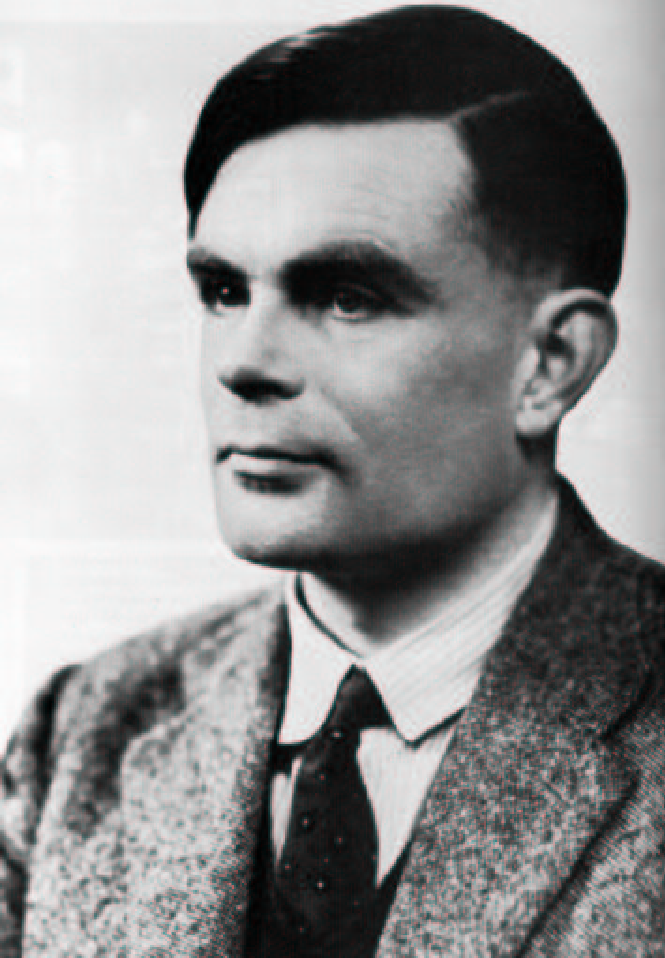
\includegraphics[width=2in]{figures/turing.pdf}}

The man pictured above is Alan Turing, the most important figure in
the history of computer science.  For decades, his fascinating life
story was shrouded by government secrecy, societal taboo, and even his
own deceptions.

At 24 Turing wrote a paper entitled \emph{On Computable Numbers, with an
Application to the Entscheidungsproblem}.  The crux of the paper was an
elegant way to model a computer in mathematical terms.  This was a
breakthrough, because it allowed the tools of mathematics to be brought to
bear on questions of computation.  For example, with his model in hand,
Turing immediately proved that there exist problems that no computer can
solve--- no matter how ingenious the programmer.  Turing's paper is all the
more remarkable because he wrote it in 1936, a full decade before any
electronic computer actually existed.

The word ``Entscheidungsproblem'' in the title refers to one of the 28
mathematical problems posed by David Hilbert in 1900 as challenges to
mathematicians of the 20th century.  Turing knocked that one off in the
same paper.  And perhaps you've heard of the ``\idx{Church-Turing
  thesis}''?  Same paper.  So Turing was obviously a brilliant guy who
generated lots of amazing ideas.  But this lecture is about one of
Turing's less-amazing ideas.  It involved codes.  It involved number
theory.  And it was sort of stupid.

%\subsection{Turing's Code}

Let's look back to the fall of 1937.  Nazi Germany was rearming under
Adolf Hitler, world-shattering war looked imminent, and--- like us--- Alan
Turing was pondering the usefulness of number theory.  He foresaw that
preserving military secrets would be vital in the coming conflict and
proposed a way \emph{to encrypt communications using number theory}.
This is an idea that has ricocheted up to our own time.  Today, number
theory is the basis for numerous public-key cryptosystems, digital
signature schemes, cryptographic hash functions, and digital cash systems.
Every time you buy a book from Amazon, check your grades on WebSIS, or use
a PayPal account, you are relying on number theoretic algorithms.
Furthermore, military funding agencies are among the biggest investors in
cryptographic research.  Sorry \idx{Hardy}!

Soon after devising his code, \idx{Turing} disappeared from public view,
and half a century would pass before the world learned the full story of
where he'd gone and what he did there.  We'll come back to Turing's life
in a little while; for now, let's investigate the code Turing left behind.
The details are uncertain, since he never formally published the idea, so
we'll consider a couple of possibilities.

\subsection{Turing's Code (Version 1.0)}

The first challenge is to translate a text message into an integer so
we can perform mathematical operations on it.  This step is not
intended to make a message harder to read, so the details are not too
important.  Here is one approach: replace each letter of the message
with two digits ($A = 01$, $B = 02$, $C = 03$, etc.) and string all
the digits together to form one huge number.  For example, the message
``victory'' could be translated this way:
%
\begin{center}
\begin{tabular}{ccccccccc}
   &``v &  i &  c &  t & o & r & y'' \\
$\rightarrow$ & 22 & 09 & 03 & 20 & 15 & 18 & 25
\end{tabular}
\end{center}
%
\idx{Turing's code} requires the message to be a prime number, so we may
need to pad the result with a few more digits to make a prime.  In
this case, appending the digits 13 gives the number 2209032015182513,
which is prime.

Now here is how the encryption process works.  In the description
below, $m$ is the unencoded message (which we want to keep secret),
$m^*$ is the encrypted message (which the Nazis may intercept), and
$k$ is the key.

\begin{description}

\item[Beforehand] The sender and receiver agree on a secret key, which
is a large prime $k$.

\item[Encryption] The sender encrypts the message $m$ by computing:
\[
m^* = m \cdot k
\]

\item[Decryption] The receiver decrypts $m^*$ by computing:
\[
\frac{m^*}{k} = \frac{m \cdot k}{k} = m
\]

\end{description}

For example, suppose that the secret key is the prime number $k =
22801763489$ and the message $m$ is ``victory''.  Then the encrypted
message is:
%
\begin{align*}
m^* & = m \cdot k \\
   & = 2209032015182513 \cdot 22801763489 \\
   & = 50369825549820718594667857
\end{align*}

There are a couple of questions that one might naturally ask about Turing's
code.

\begin{enumerate}

\item How can the sender and receiver ensure that $m$ and $k$ are
prime numbers, as required?

The general problem of determining whether a large number is prime or
composite has been studied for centuries, and reasonably good primality
tests were known even in Turing's time.  In 2002, Manindra Agrawal, Neeraj
Kayal, and Nitin Saxena announced a primality test that is guaranteed to
work on a number $n$ in about $(\log n)^{12}$ steps, that is, a number of
steps bounded by a twelfth degree polynomial in the length (in bits) of
the input, $n$.  This definitively places primality testing way below the
problems of exponential difficulty.  Amazingly, the description of their
breakthrough algorithm was only thirteen lines long!

Of course, a twelfth degree polynomial grows pretty fast, so the
Agrawal,\emph{ et al.}\ procedure is of no practical use.  Still, good
ideas have a way of breeding more good ideas, so there's certainly hope
further improvements will lead to a procedure that is useful in practice.
But the truth is, there's no practical need to improve it, since very
efficient \emph{probabilistic} procedures for prime-testing have been
known since the early 1970's.  These procedures have some probability of
giving a wrong answer, but their probability of being wrong is so tiny
that betting on their answers is the best bet you'll ever make.

\item Is Turing's code secure?

The Nazis see only the encrypted message $m^* = m \cdot k$, so
recovering the original message $m$ requires factoring $m^*$.  Despite
immense efforts, no really efficient factoring algorithm has ever been
found.  It appears to be a fundamentally difficult problem, though a
breakthrough someday is not impossible.  In effect, Turing's code puts
to practical use his discovery that there are limits to the power of
computation.  Thus, provided $m$ and $k$ are sufficiently large, the
Nazis seem to be out of luck!

\end{enumerate}

This all sounds promising, but there is a major flaw in Turing's code.

\subsection{Breaking Turing's Code}

Let's consider what happens when the sender transmits a
\emph{second} message using Turing's code and the same key.  This
gives the Nazis two encrypted messages to look at:
%
\[
m_1^* = m_1 \cdot k
\hspace{0.75in} \text{and} \hspace{0.75in}
m_2^* = m_2 \cdot k
\]
%
The greatest common divisor of the two encrypted messages, $m_1^*$ and
$m_2^*$, is the secret key $k$.  And, as we've seen, the $\gcd$ of two
numbers can be computed very efficiently.  So after the second message is
sent, the Nazis can recover the secret key and read \emph{every}
message!

It is difficult to believe a mathematician as brilliant as Turing
could overlook such a glaring problem.  One possible explanation is
that he had a slightly different system in mind, one based on
\emph{modular} arithmetic.

%% Problems %%%%%%%%%%%%%%%%%%%%%%%%%%%%%%%%%%%%%%%%%%%%%%%%%%%%%%%%%%%%%%%%%%%
%\startclassproblems
%\pinput{CP_}


%% Modular Arithmetic %%%%%%%%%%%%%%%%%%%%%%%%%%%%%%%%%%%%%%%%%%%%%%%%%%%%%%%%%
\hyperdef{modular}{arithmetic}{\section{Modular Arithmetic}}
\label{modular_arithmeric_sec}

% Congruence is a weak form of equality.

On page 1 of his masterpiece on number theory, \emph{Disquisitiones
  Arithmeticae}, \idx{Gauss} introduced the notion of
``\idx{congruence}''.  Now, Gauss is another guy who managed to cough up a
half-decent idea every now and then, so let's take a look at this one.
Gauss said that $a$ is \term{congruent} to $b$ \term{modulo} $n$ iff $n
\divides (a - b)$.  This is denoted $a$ \index{$\equiv \pmod{n}$} $b
\pmod{n}$.  For example:
%
\[
29 \equiv 15 \pmod{7}  \quad\text{ because }  7 \divides (29 - 15).
\]

There is a close connection between congruences and remainders:
\begin{lemma}[Congruences and Remainders]
\label{lem:conrem}
\[
a \equiv b \pmod{n} \qiff \rem{a}{n} = \rem{b}{n}.
\]
\end{lemma}

\begin{proof}
By the Division Theorem, there exist unique pairs of integers $q_1, r_1$
and $q_2, r_2$ such that:
%
\begin{align*}
a & = q_1 n + r_1 & \text{where $0 \leq r_1 < n$}, \\
b & = q_2 n + r_2 & \text{where $0 \leq r_2 < n$}.
\end{align*}
%
In these terms, $\rem{a}{n} = r_1$ and $\rem{b}{n} = r_2$.
Subtracting the second equation from the first gives:
%
\begin{align*}
a - b & = (q_1 - q_2) n + (r_1 - r_2)
  & \text{where $-n < r_1 - r_2 < n$}.
\end{align*}
%
Now $a \equiv b \pmod{n}$ if and only if $n$ divides the left side.
This is true if and only if $n$ divides the right side, which holds if
and only if $r_1 - r_2$ is a multiple of $n$.  Given the bounds on
$r_1 - r_2$, this happens precisely when $r_1 = r_2$, which is
equivalent to $\rem{a}{n} = \rem{b}{n}$.
\end{proof}

So we can also see that
\[
29 \equiv 15 \pmod{7} \quad\text{ because } \rem{29}{7} = 1 = \rem{15}{7}.
\]
This formulation explains why the congruence relation has properties like
an equality relation.  Notice that even though (mod 7) appears over on the
right side the $\equiv$ symbol, it is in no sense more strongly associated
with the 15 than the 29.  It would really be clearer to write $29
\equiv_{\mod 7} 15$ for example, but the notation with the modulus at the
end is firmly entrenched and we'll stick to it.

We'll make frequent use of the following immediate Corollary of
Lemma~\ref{lem:conrem}:
\begin{corollary}\label{aran}
\[
a \equiv \rem{a}{n} \pmod{n}
\]
\end{corollary}

Still another way to think about congruence modulo $n$ is that it
\emph{defines a partition of the integers into $n$ sets so that congruent
numbers are all in the same set}.  For example, suppose that we're working
modulo 3.  Then we can partition the integers into 3 sets as follows:
%
\[
\begin{array}{cccccccccc}
\{ & \dots, & -6, & -3, & 0, & 3, & 6, & 9, & \dots & \} \\
\{ & \dots, & -5, & -2, & 1, & 4, & 7, & 10, & \dots & \} \\
\{ & \dots, & -4, & -1, & 2, & 5, & 8, & 11, & \dots & \}
\end{array}
\]
according to whether their remainders on division by 3 are 0, 1, or 2.
The upshot is that when arithmetic is done modulo $n$ there are really
only $n$ different kinds of numbers to worry about, because there are only
$n$ possible remainders.  In this sense, modular arithmetic is a
simplification of ordinary arithmetic and thus is a good reasoning tool.

There are many useful facts about congruences, some of which are listed in
the lemma below.  The overall theme is that \emph{congruences work a lot
like equations}, though there are a couple of exceptions.

\begin{lemma}[Facts About Congruences]  The following  hold for 
$n \geq 1$:
%
\begin{enumerate}
\item $a \equiv a \pmod{n}$
\item $a \equiv b \pmod{n}$ implies $b \equiv a \pmod{n}$
\item $a \equiv b \pmod{n}$ and $b \equiv c \pmod{n}$ implies $a \equiv c \pmod{n}$
\item $a \equiv b \pmod{n}$ implies $a + c \equiv b + c \pmod{n}$
\item $a \equiv b \pmod{n}$ implies $a c \equiv b c \pmod{n}$
\item $a \equiv b \pmod{n}$ and $c \equiv d \pmod{n}$ imply $a + c
\equiv b + d \pmod{n}$
\item $a \equiv b \pmod{n}$ and $c \equiv d \pmod{n}$ imply $a c
\equiv b d \pmod{n}$
\end{enumerate}
\end{lemma}

\begin{proof}
Parts 1.--3.\ follow immediately from Lemma~\ref{lem:conrem}.  Part 4.\
follows immediately from the definition that $a \equiv b \pmod{n}$ iff $n
\divides (a-b)$.  Likewise, part 5.\ follows because if $n \divides (a-b)$
then it divides $(a-b)c = ac - bc$.  To prove part 6., assume
\begin{equation}\label{ab}
a \equiv b \pmod{n}
\end{equation}
and
\begin{equation}\label{cd}
c \equiv d \pmod{n}.
\end{equation}
Then
\begin{align*}
a + c & \equiv b + c \pmod{n} & \text{(by part 4.\ and~\eqref{ab}}),\\
c + b & \equiv d + b \pmod{n} & \text{(by part 4.\ and~\eqref{cd}), so}\\
b + c & \equiv b + d \pmod{n} & \text{and therefore}\\
a + c & \equiv b + d \pmod{n} & \text{(by part 3.)}
\end{align*}
Part 7.\ has a similar proof.
\end{proof}

\iffalse

There is a close connection between modular arithmetic and the
remainder operation, which we looked at last time.  To clarify this
link, let's reconsider the partition of the integers defined by
congruence modulo 3:
%
\[
\begin{array}{cccccccccc}
\{ & \dots, & -6, & -3, & 0, & 3, & 6, & 9, & \dots & \} \\
\{ & \dots, & -5, & -2, & 1, & 4, & 7, & 10, & \dots & \} \\
\{ & \dots, & -4, & -1, & 2, & 5, & 8, & 11, & \dots & \}
\end{array}
\]
%
Notice that two numbers are in the same set if and only if they leave
the same remainder when divided by 3.  The numbers in the first set
all leave a remainder of 0 when divided by 3, the numbers in the
second set leave a remainder of 1, and the numbers in the third leave
a remainder of 2.  Furthermore, notice that each number is in the same
set as its own remainder.  For example, 11 and $\rem{11}{3} = 2$ are
both in the same set.  Let's bundle all this happy goodness into a
lemma.
\fi

%\TBA{put in 'example' environment}

\subsection{\idx{Turing's Code} (Version 2.0)}

In 1940 France had fallen before Hitler's army, and Britain alone stood
against the Nazis in western Europe.  British resistance depended on a
steady flow of supplies brought across the north Atlantic from the United
States by convoys of ships.  These convoys were engaged in a cat-and-mouse
game with German ``U-boats'' ---submarines ---which prowled the Atlantic,
trying to sink supply ships and starve Britain into submission.  The
outcome of this struggle pivoted on a balance of information: could the
Germans locate convoys better than the Allies could locate U-boats or vice
versa?

Germany lost.

But a critical reason behind Germany's loss was made public only in
1974: the British had broken Germany's naval code, Enigma.  Through
much of the war, the Allies were able to route convoys around German
submarines by listening into German communications.  The British
government didn't explain \emph{how} Enigma was broken until 1996.
When the analysis was finally released (by the US), the author was
none other than Alan Turing.  In 1939 he had joined the secret British
codebreaking effort at Bletchley Park.  There, he played a central
role in cracking the German's Enigma code and thus in preventing
Britain from falling into Hitler's hands.

Governments are always tight-lipped about cryptography, but the
half-century of official silence about Turing's role in breaking
Enigma and saving Britain may be related to some disturbing events
after the war.

Let's consider an alternative interpretation of Turing's code.
Perhaps we had the basic idea right (multiply the message by the key),
but erred in using \emph{conventional} arithmetic instead of
\emph{modular} arithmetic.  Maybe this is what Turing meant:
%
\begin{description}

\item[Beforehand] The sender and receiver agree on a large prime $p$,
which may be made public.  (This will be the modulus for all our
arithmetic.)  They also agree on a secret key $k \in \set{1, 2,
\dots, p-1}$.

\item[Encryption] The message $m$ can be any integer in the set
$\set{0, 1, 2, \dots, p-1}$; in particular, the message is no longer
required to be a prime.  The sender encrypts the message $m$ to
produce $m^*$ by computing:
%
\begin{equation}
m^* = \rem{mk}{p} \label{eq:turing-code}
\end{equation}

\item[Decryption] (Uh-oh.)

\end{description}

The decryption step is a problem.  We might hope to decrypt in the
same way as before: by dividing the encrypted message $m^*$ by the key
$k$.  The difficulty is that $m^*$ is the \emph{remainder} when $mk$
is divided by $p$.  So dividing $m^*$ by $k$ might not even give us an
integer!

This decoding difficulty can be overcome with a better understanding
of arithmetic modulo a prime.

%% Problems %%%%%%%%%%%%%%%%%%%%%%%%%%%%%%%%%%%%%%%%%%%%%%%%%%%%%%%%%%%%%%%%%%%
\begin{problems}
\classproblems
\pinput{CP_proving_basic_congruence_properties}
\pinput{CP_multiples_of_9_and_11}
\pinput{CP_13th_roots}
\end{problems}

%% Arithmetic with a Prime Modulus %%%%%%%%%%%%%%%%%%%%%%%%%%%%%%%%%%%%%%%%%%%%
\section{Arithmetic with a Prime Modulus}\label{mod_prime_sec}

\subsection{\idx{Multiplicative Inverses}}
\label{sec:prime}

The \term{multiplicative inverse} of a number $x$ is another number
$x^{-1}$ such that:
%
\[
x \cdot x^{-1} = 1
\]

Generally, multiplicative inverses exist over the real numbers.  For
example, the multiplicative inverse of 3 is $1 / 3$ since:
%
\[
3 \cdot \frac{1}{3} = 1
\]
%
The sole exception is that 0 does not have an inverse.

On the other hand, inverses generally do not exist over the integers.
For example, 7 can not be multiplied by another integer to give 1.

Surprisingly, multiplicative inverses do exist when we're working
\emph{modulo a prime number}.  For example, if we're working modulo
5, then 3 is a multiplicative inverse of 7, since:
%
\[
7 \cdot 3 \equiv 1 \pmod{5}
\]
%
(All numbers congruent to 3 modulo 5 are also multiplicative inverses
of 7; for example, $7 \cdot 8 \equiv 1 \pmod{5}$ as well.)  The only
exception is that numbers congruent to 0 modulo 5 (that is, the
multiples of 5) do not have inverses, much as 0 does not have an
inverse over the real numbers.  Let's prove this.

\begin{lemma}
\label{lem:inverses}
If $p$ is prime and $k$ is not a multiple of $p$, then $k$ has a
multiplicative inverse.
\end{lemma}

\begin{proof}
Since $p$ is prime, it has only two divisors: 1 and $p$.  And since
$k$ is not a multiple of $p$, we must have $\gcd(p, k) = 1$.
Therefore, there is a linear combination of $p$ and $k$ equal to 1:
%
\[
s p + t k = 1
\]
%
Rearranging terms gives:
%
\[
s p = 1 - t k
\]
%
This implies that $p \divides \paren{1 - tk}$ by the definition of divisibility,
and therefore $tk \equiv 1 \pmod{p}$ by the definition of congruence.
Thus, $t$ is a multiplicative inverse of $k$.
\end{proof}

Multiplicative inverses are the key to decryption in Turing's code.
Specifically, we can recover the original message by multiplying the
encoded message by the \emph{inverse} of the key:
\begin{align*}
m^* \cdot k^{-1}
    & = \rem{mk}{p} \cdot k^{-1}
         & \text{(def.~\eqref{eq:turing-code} of $m^*$)}\\
    & \equiv (mk)k^{-1} \pmod{p} & \text{(by Cor.~\ref{aran})}\\
    & \equiv m \pmod{p}.
\end{align*}

This shows that $m^* k^{-1}$ is congruent to the original message $m$.
Since $m$ was in the range $0, 1, \dots, p - 1$, we can recover
it exactly by taking a remainder:
%
\[
m = \rem{m^* k^{-1}}{p}
\]
%
So now we can decrypt!

\subsection{\idx{Cancellation}}

Another sense in which real numbers are nice is that one can cancel
multiplicative terms.  In other words, if we know that $m_1 k = m_2 k$,
then we can cancel the $k$'s and conclude that $m_1 = m_2$, provided $k
\neq 0$.  In general, cancellation is \emph{not} valid in modular
arithmetic.  For example, this congruence is correct:
%
\[
2 \cdot 3 \equiv 4 \cdot 3 \pmod{6}
\]
%
But if we cancel the 3's, we reach a false conclusion:
%
\[
2 \equiv 4 \pmod{6}
\]
%
The fact that multiplicative terms can not be cancelled is the most
significant sense in which congruences differ from ordinary equations.
However, this difference goes away if we're working modulo a
\emph{prime}; then cancellation is valid.

\begin{lemma}
\label{lem:cancel}
Suppose $p$ is a prime and $k$ is not a multiple of $p$.  Then
%
\[
ak \equiv bk \pmod{p}
\hspace{0.5in} \text{implies} \hspace{0.5in}
a \equiv b \pmod{p}
\]
\end{lemma}

\begin{proof}
Multiply both sides of the congruence by $k^{-1}$.
\end{proof}

We can use this lemma to get a bit more insight into how Turing's code
works.  In particular, the encryption operation in Turing's code
\emph{permutes the set of possible messages}.  This is stated more
precisely in the following corollary.

\hyperdef{for}{Fermat}{\begin{corollary}
\label{cor:prime-permutes}
Suppose $p$ is a prime and $k$ is not a multiple of $p$.  Then the
sequence:
\[
\rem{(0 \cdot k)}{p},\quad
\rem{(1 \cdot k)}{p},\quad
\rem{(2 \cdot k)}{p},\quad
 \dots,\quad
\rem{\paren{(p-1) \cdot k}}{p}
\]
is a permutation\footnote{A \term{permutation} of a sequence of elements
is a sequence with the same elements (including repeats) possibly in a
different order.  More formally, if
\[
\vec{e} \eqdef e_1,e_2,\dots,e_n
\]
is a length $n$ sequence, and  $\pi: \set{1,\dots, n} \to \set{1,\dots,
n}$ is a bijection, then
\[
e_{\pi(1)}, e_{\pi(2)},\dots, e_{\pi(n)},
\]
is a \emph{permutation} of $\vec{e}$.} of the sequence:
\[
0,\quad 1,\quad 2,\quad \dots,\quad (p - 1)
\]
This remains true if the first term is deleted from each sequence.
\end{corollary}}

\begin{proof}
The first sequence contains $p$ numbers, which are all in the range
$0$ to $p - 1$ by the definition of remainder.  Furthermore, the
numbers in the first sequence are all different; by
Lemma~\ref{lem:cancel}, $i k \equiv j k \pmod{p}$
if and only if $i \equiv j \pmod{p}$, and no two numbers in the range 0, 1,
\dots, p - 1 are congruent modulo $p$.  Thus, the first sequence must
contain \emph{all} of the numbers from 0 to $p - 1$ in some order.
The claim remains true if the first terms are deleted, because both
sequences begin with 0.
\end{proof}

For example, suppose $p = 5$ and $k = 3$.  Then the sequence:
%
\[
\underbrace{\rem{(0 \cdot 3)}{5}}_{=0},\quad
\underbrace{\rem{(1 \cdot 3)}{5}}_{=3},\quad
\underbrace{\rem{(2 \cdot 3)}{5}}_{=1},\quad
\underbrace{\rem{(3 \cdot 3)}{5}}_{=4},\quad
\underbrace{\rem{(4 \cdot 3)}{5}}_{=2}
\]
%
is a permutation of 0, 1, 2, 3, 4 and the last four terms are a
permutation of 1, 2, 3, 4.  As long as the Nazis don't know the secret key
$k$, they don't know how the set of possible messages are permuted by the
process of encryption and thus can't read encoded messages.

%%%%%%%%%%%%%%%%%%%%%%%%%%%%%%%%%%%%%%%%%%%%%%%%%%%%%%%%%%%%%%%%%%%%%%%%%%%%%%%

\subsection{Fermat's Little Theorem}

A remaining challenge in using Turing's code is that decryption requires
the inverse of the secret key $k$.  An effective way to calculate
$k^{-1}$ follows from the proof of Lemma~\ref{lem:inverses}: $k^{-1} =
\rem{t}{p}$ where $s,t$ are coefficients such that $sp+tk=1$.  Notice that
$t$ is easy to find using the Pulverizer.

An alternative approach, about equally efficient and probably more
memorable, is to rely on Fermat's Little Theorem, which is much easier than his
famous Last Theorem.  \iffalse ---and more useful.\fi


\begin{theorem}[\idx{Fermat's Little Theorem}]\label{fermat_little}
Suppose $p$ is a prime and $k$ is not a multiple of $p$.  Then:
%
\[
k^{p-1} \equiv 1 \pmod{p}
\]
\end{theorem}

\begin{proof}
We reason as follows:
\begin{align*}
1 \cdot 2 \cdots (p-1)
	& = \rem{k}{p} \cdot \rem{2k}{p} \cdots
	\rem{(p-1)k}{p} & \text{(by Cor~\ref{cor:prime-permutes})}\\
	& \equiv k \cdot 2k \cdots (p-1) k \pmod{p}
            & \text{(by Cor~\ref{aran})}\\
	& \equiv (p-1)! \cdot k^{p-1} \pmod{p} & \text{(rearranging terms)}\\
\end{align*}

Now $(p - 1)!$ can not be a multiple of $p$, because the prime
factorizations of $1, 2, \dots, (p - 1)$ contain only primes smaller
than $p$.  Therefore, we can cancel $(p - 1)!$ from the first
expression and the last by Lemma~\ref{lem:cancel}, which proves the
claim.
\end{proof}

Here is how we can find inverses using Fermat's Theorem.  Suppose $p$
is a prime and $k$ is not a multiple of $p$.  Then, by Fermat's
Theorem, we know that:
%
\[
k^{p-2} \cdot k \equiv 1 \pmod{p}
\]
%
Therefore, $k^{p-2}$ must be a multiplicative inverse of $k$.  For
example, suppose that we want the multiplicative inverse of 6 modulo
17.  Then we need to compute $\rem{6^{15}}{17}$, which we can do by
successive squaring.  All the congruences below hold modulo 17.
%
\begin{align*}
6^2 & \equiv 36 \equiv 2 \\
6^4 & \equiv (6^2)^2 \equiv 2^2 \equiv 4 \\
6^8 & \equiv (6^4)^2 \equiv 4^2 \equiv 16 \\
6^{15} & \equiv 6^8 \cdot 6^4 \cdot 6^2 \cdot 6
       \equiv 16 \cdot 4 \cdot 2 \cdot 6
       \equiv 3
\end{align*}
%
Therefore, $\rem{6^{15}}{17} = 3$.  Sure enough, 3 is the multiplicative
inverse of 6 modulo 17, since:
%
\[
3 \cdot 6 \equiv 1 \pmod{17}
\]

In general, if we were working modulo a prime $p$, finding a
multiplicative inverse by trying every value between 1 and $p - 1$
would require about $p$ operations.  However, the approach above
requires only about $\log p$ operations, which is far better when $p$
is large.

\subsection{Breaking \idx{Turing's Code} ---Again}

The Germans didn't bother to encrypt their weather reports with the
highly-secure Enigma system.  After all, so what if the Allies learned
that there was rain off the south coast of Iceland?  But, amazingly, this
practice provided the British with a critical edge in the Atlantic naval
battle during 1941.

The problem was that some of those weather reports had originally been
transmitted from U-boats out in the Atlantic.  Thus, the British
obtained both unencrypted reports and the same reports encrypted with
Enigma.  By comparing the two, the British were able to determine
which key the Germans were using that day and could read all other
Enigma-encoded traffic.  Today, this would be called a
\term{known-plaintext attack}.

Let's see how a known-plaintext attack would work against Turing's
code.  Suppose that the Nazis know both $m$ and $m^*$ where:
%
\[
m^* \equiv mk \pmod{p}
\]
%
Now they can compute:
%
\begin{align*}
m^{p-2} \cdot m^*
  & = m^{p-2} \cdot \rem{mk}{p}
                & \text{(def.~\eqref{eq:turing-code} of $m^*$)}\\
  & \equiv m^{p-2} \cdot mk \pmod{p} & \text{(by Cor~\ref{aran})}\\
  & \equiv m^{p-1} \cdot k \pmod{p}\\ % & \text{(simplification)}\\
  & \equiv k \pmod{p} & \text{(Fermat's Theorem)}
\end{align*}
%
Now the Nazis have the secret key $k$ and can decrypt any message!

This is a huge vulnerability, so Turing's code has no practical value.
Fortunately, Turing got better at cryptography after devising this
code; his subsequent cracking of Enigma surely saved thousands of
lives, if not the whole of Britain.

%  I could insert a bit about public-key cryptography here as introduction to
%  the recitation.

\subsection{Turing Postscript}

A few years after the war, Turing's home was robbed.  Detectives soon
determined that a former homosexual lover of Turing's had conspired in the
robbery.  So they arrested him ---that is, they arrested Alan Turing
---because homosexuality was a British crime punishable by up to two years
in prison at that time.  Turing was sentenced to a humiliating hormonal
``treatment'' for his homosexuality: he was given estrogen injections.  He
began to develop breasts.

Three years later, Alan \idx{Turing}, the founder of computer science, was
dead.  His mother explained what happened in a biography of her own
son.  Despite her repeated warnings, Turing carried out chemistry
experiments in his own home.  Apparently, her worst fear was realized:
by working with potassium cyanide while eating an apple, he poisoned
himself.

However, Turing remained a puzzle to the very end.  His mother was a
devoutly religious woman who considered suicide a sin.  And, other
biographers have pointed out, Turing had previously discussed
committing suicide by eating a poisoned apple.  Evidently, Alan
Turing, who founded computer science and saved his country, took his
own life in the end, and in just such a way that his mother could
believe it was an accident.

Turing's last project before he disappeared from public view in 1939
involved the construction of an elaborate mechanical device to test a
mathematical conjecture called the Riemann Hypothesis.  This conjecture
first appeared in a sketchy paper by Berhard Riemann in 1859 and is now
one of the most famous unsolved problem in mathematics.

\floatingtextbox{
\textboxtitle{The \idx{Riemann Hypothesis}}

The formula for the sum of an infinite geometric series says:
\[
1 + x + x^2 + x^3 + \cdots = \frac{1}{1-x}
\]
Substituting $x = \frac{1}{2^s}$, $x = \frac{1}{3^s}$, 
$x = \frac{1}{5^s}$, and so on for each prime
number gives a sequence of equations:
%
\begin{align*}
1 + \frac{1}{2^s} + \frac{1}{2^{2s}} + \frac{1}{2^{3s}} + \cdots
    & = \frac{1}{1 - 1 / 2^s} \\
1 + \frac{1}{3^s} + \frac{1}{3^{2s}} + \frac{1}{3^{3s}} + \cdots
    & = \frac{1}{1 - 1 / 3^s} \\
1 + \frac{1}{5^s} + \frac{1}{5^{2s}} + \frac{1}{5^{3s}} + \cdots
    & = \frac{1}{1 - 1 / 5^s} \\
    & \text{etc.}
\end{align*}
%
Multiplying together all the left sides and all the right sides gives:
%
\[
\sum_{n=1}^{\infty} \frac{1}{n^s} = \prod_{p \in \text{primes}} \paren{\frac{1}{1 - 1 / p^s}}
\]
%
The sum on the left is obtained by multiplying out all the infinite
series and applying the Fundamental Theorem of Arithmetic.  For
example, the term $1 / 300^s$ in the sum is obtained by multiplying $1
/ 2^{2s}$ from the first equation by $1 / 3^s$ in the second and $1 /
5^{2s}$ in the third.  Riemann noted that every prime appears in the
expression on the right.  So he proposed to learn about the primes by
studying the equivalent, but simpler expression on the left.  In
particular, he regarded $s$ as a complex number and the left side as a
function, $\zeta(s)$.  Riemann found that the distribution of primes
is related to values of $s$ for which $\zeta(s) = 0$, which led to his
famous conjecture:
\begin{quote}
  \term{The Riemann Hypothesis}: Every nontrivial zero of the zeta
  function $\zeta(s)$ lies on the line $s = 1/2 + c i$ in the complex
  plane.
\end{quote}

Researchers continue to work intensely to settle this conjecture, as they
have for over a century.  A proof would immediately imply, among other
things, a strong form of the \idx{Prime Number Theorem} ---and earn the
prover a \$1 million prize!  (We're not sure what the cash would be for a
counter-example, but the discoverer would be wildly applauded by
mathematicians everywhere.)}

%% Problems %%%%%%%%%%%%%%%%%%%%%%%%%%%%%%%%%%%%%%%%%%%%%%%%%%%%%%%%%%%%%%%%%%%
\begin{problems}
\classproblems
\pinput{CP_nonparallel_lines}
\pinput{CP_Sk_equiv_-1_mod_p}

\homeworkproblems
\pinput{PS_calculating_inverses}
\end{problems}

%% Arithmetic with an Arbitrary Modulus %%%%%%%%%%%%%%%%%%%%%%%%%%%%%%%%%%%%%%%
\hyperdef{mod}{n}{\section{Arithmetic with an Arbitrary
    Modulus}}\label{arithmetic_modn_sec}

Turing's code did not work as he hoped.  However, his essential
idea--- using number theory as the basis for cryptography--- succeeded
spectacularly in the decades after his death.

In 1977, Ronald \idx{Rivest}, Adi \idx{Shamir}, and Leonard \idx{Adleman}
at MIT proposed a highly secure cryptosystem (called \textbf{\idx{RSA}})
based on number theory.  Despite decades of attack, no significant
weakness has been found.  Moreover, RSA has a major advantage over
traditional codes: the sender and receiver of an encrypted message need
not meet beforehand to agree on a secret key.  Rather, the receiver has
both a \term{secret key}, which she guards closely, and a \term{public
  key}, which she distributes as widely as possible.  To send her a
message, one encrypts using her widely-distributed public key.  Then she
decrypts the message using her closely-held private key.  The use of such
a \term{public key cryptography} system allows you and Amazon, for
example, to engage in a secure transaction without meeting up beforehand
in a dark alley to exchange a key.

Interestingly, RSA does not operate modulo a prime, as Turing's scheme
may have, but rather modulo the product of \emph{two} large primes.
Thus, we'll need to know a bit about how arithmetic works modulo a
composite number in order to understand RSA.  Arithmetic modulo an
arbitrary positive integer is really only a little more painful than
working modulo a prime, in the same sense that a doctor says ``This is
only going to hurt a little'' before he jams a big needle in your arm.

\subsection{Relative Primality and Phi}

First, we need a new definition.  Integers $a$ and $b$ are
\term{relatively prime} iff $\gcd(a, b) = 1$.  For example, 8 and 15
are relatively prime, since $\gcd(8, 15) = 1$.  Note that every
integer is relatively prime to a genuine prime number $p$, except for
multiples of $p$.

We'll also need a certain function that is defined using relative
primality.  Let $n$ be a positive integer.  Then $\phi(n)$ denotes the
number of integers in $\set{1, 2, \dots, n - 1}$ that are relatively prime
to $n$.  For example, $\phi(7) = 6$, since 1, 2, 3, 4, 5, and 6 are all
relatively prime to 7.  Similarly, $\phi(12) = 4$, since only 1, 5, 7, and
11 are relatively prime to 12.  If you know the prime factorization of
$n$, then computing $\phi(n)$ is a piece of cake, thanks to the following
theorem.  The function $\phi$ is known as \term{Euler's $\phi$ function};
it's also called Euler's \emph{\idx{totient}} function.

\begin{theorem}
\label{th:phi}
The function $\phi$ obeys the following relationships:
\begin{enumerate}
\item[(a)] If $a$ and $b$ are relatively prime, then $\phi(ab) = \phi(a)\phi(b)$.
\item[(b)] If $p$ is a prime, then $\phi(p^k) = p^k - p^{k-1}$ for $k \geq 1$.
\end{enumerate}
\end{theorem}

Here's an example of using Theorem~\ref{th:phi} to compute $\phi(300)$:
%
\begin{align*}
\phi(300)
    & = \phi(2^2 \cdot 3 \cdot 5^2)\\
    & = \phi(2^2) \cdot \phi(3) \cdot \phi(5^2)
            & \text{(by Theorem~\ref{th:phi}.(a))}\\
    & = (2^2 - 2^1) (3^1 - 3^0) (5^2 - 5^1) 
            & \text{(by Theorem~\ref{th:phi}.(b))}\\
    & = 80.
\end{align*}
\iffalse
We factor 300 in the first step, use part (1) of Theorem~\ref{th:phi}
twice in the second step, use part (2) in the third step, and then
simplify.
\fi

The proof of Theorem~\ref{th:phi}.(a) requires a few more properties of
modular arithmetic worked out in the next section (see
Problem~\ref{PS_Euler_function_multiplicativity}).  We'll also give
another a proof in a few weeks based on rules for counting things.

To prove Theorem~\ref{th:phi}.(b), notice that the numbers in the interval
from 0 to $p^{k}-1$ that are divisible by $p$ are all those of the form
$mp$.  For $mp$ to be in the interval, $m$ can take any value from 0 to
$p^{k-1}-1$ and no others, so there are exactly $p^{k-1}$ numbers in the
interval that are divisible by $p$.  Now $\phi(p^{k})$ equals the number
of remaining elements in the interval, namely, $p^k -p^{k-1}$.


\subsection{Generalizing to an Arbitrary Modulus}

Let's generalize what we know about arithmetic modulo a prime.  Now,
instead of working modulo a prime $p$, we'll work modulo an arbitrary
positive integer $n$.  The basic theme is that arithmetic modulo $n$ may
be complicated, but the integers {\em relatively prime} to $n$ remain
fairly well-behaved.  For example, the proof of Lemma~\ref{lem:inverses}
of an inverse for $k$ modulo $p$ extends to an inverse for $k$ relatively
prime to $n$:

\begin{lemma}
\label{lem:inverse-arb}
Let $n$ be a positive integer.  If $k$ is relatively prime to $n$,
then there exists an integer $k^{-1}$ such that:
%
\[
k \cdot k^{-1} \equiv 1 \pmod{n}
\]
\end{lemma}


\iffalse
\begin{proof}
There exist integers $s$ and $t$ such that $s k + t n = \gcd(k, n) =
1$ by Theorem~\ref{th:gcd}.  Rearranging terms gives $tn = 1 - sk$,
which implies that $n \divides 1 - sk$ and $sk \equiv 1 \pmod{n}$.  Define
$k^{-1}$ to be $s$.
\end{proof}
\fi

As a consequence of this lemma, we can cancel a multiplicative term
from both sides of a congruence if that term is relatively prime to
the modulus:

\begin{corollary}
\label{cor:cancellation-arb}
Suppose $n$ is a positive integer and $k$ is relatively prime to $n$.
If
%
\[
a k \equiv b k \pmod{n}
\]
%
then
%
\[
a \equiv b \pmod{n}
\]
\end{corollary}

This holds because we can multiply both sides of the first congruence
by $k^{-1}$ and simplify to obtain the second.

\subsection{Euler's Theorem}

\idx{RSA} essentially relies on \idx{Euler's Theorem}, a generalization of
Fermat's Theorem to an arbitrary modulus.  The proof is much like the
proof of Fermat's Theorem, except that we focus on integers relatively
prime to the modulus.  Let's start with a lemma.

\begin{lemma}
\label{lem:permutes-arb}
Suppose $n$ is a positive integer and $k$ is relatively prime to $n$.
Let $k_1, \dots, k_r$ denote all the integers relatively prime to $n$
in the range $0 \leq k_i < n$.  Then the sequence:
%
\[
\rem{k_1 \cdot k}{n},\quad
\rem{k_2 \cdot k}{n},\quad
\rem{k_3 \cdot k}{n},\quad
\quad \dots\quad,
\rem{k_r \cdot k}{n}
\]
%
is a permutation of the sequence:
%
\[
k_1,\quad k_2,\quad \dots\quad, k_r.
\]
\end{lemma}

\begin{proof}
We will show that the numbers in the first sequence are all distinct
and all appear in the second sequence.  Since the two sequences have
the same length, the first must be a permutation of the second.

First, we show that the numbers in the first sequence are all
distinct.  Suppose that $\rem{k_i k}{n} = \rem{k_j k}{n}$.  This is
equivalent to $k_i k \equiv k_j k \pmod{n}$, which implies $k_i \equiv
k_j \pmod{n}$ by Corollary~\ref{cor:cancellation-arb}.  This, in turn,
means that $k_i = k_j$ since both are between 1 and $n-1$.  Thus, a
term in the first sequence is not equal to any other term.

Next, we show that each number in the first sequence appears in the
second.  By assumption, $\gcd(k_i, n) = 1$ and $\gcd(k, n) = 1$, which
means that
%
\begin{align*}
\gcd(n, \rem{k_i k}{n}) & = \gcd(k_i k, n)
            & \text{(by Lemma~\ref{lem:gcd}.\ref{gcd5})}\\
      & = 1 & \text{(by Lemma~\ref{lem:gcd}.\ref{gcd3})}.
\end{align*}
%
So $\rem{k_i k}{n}$ is relatively prime to $n$ and is in the range from 0
to $n - 1$ by the definition of remainder.  The second sequence is defined
to consist of all such integers.
\end{proof}

We can now prove Euler's Theorem:

\begin{theorem}[\idx{Euler's Theorem}]
Suppose $n$ is a positive integer and $k$ is relatively prime to $n$.
Then
\begin{eqnarray*}
k^{\phi(n)} \equiv 1 \pmod{n}
\end{eqnarray*}
\end{theorem}

\begin{proof}
Let $k_1, \dots, k_r$ denote all integers relatively prime to $n$
such that $0 \leq k_i < n$.  Then $r = \phi(n)$, by the definition of
the function $\phi$.  Now we can reason as follows:
%
\begin{align*}
\lefteqn{k_1 \cdot k_2 \cdots k_r} \hspace{0.25in} \\
& =
\rem{k_1 \cdot k}{n} \cdot 
\rem{k_2 \cdot k}{n} \cdots 
\rem{k_r \cdot k}{n} & \text{(by Lemma~\ref{lem:permutes-arb})}
\\
& \equiv 
(k_1 \cdot k) \cdot 
(k_2 \cdot k) \cdot 
\cdots 
(k_r \cdot k) \pmod{n} & \text{(by Cor~\ref{aran})}
\\
& \equiv  
(k_1 \cdot k_2 \cdots k_r) \cdot k^r \pmod{n} & \text{(rearranging terms)}
\end{align*}

Lemma~\ref{lem:gcd}.\ref{gcd3}.\ implies that $k_1 \cdot k_2
\cdots k_r$ is prime relative to $n$.  Therefore, we can cancel this
product from the first expression and the last by
Corollary~\ref{cor:cancellation-arb}.  This proves the claim.
\end{proof}

We can find multiplicative inverses using Euler's theorem as we did
with Fermat's theorem: if $k$ is relatively prime to $n$, then
$k^{\phi(n) - 1}$ is a multiplicative inverse of $k$ modulo $n$.
However, this approach requires computing $\phi(n)$.  Our best method
for doing so requires factoring $n$, which can be quite difficult in
general.  Fortunately, when we know how to factor $n$, we can
use Theorem~\ref{th:phi} to compute $\phi(n)$ efficiently!


\subsection{RSA}
Finally, we are ready to see how the \term{RSA public key encryption
  scheme} works:
\begin{center}
RSA Public Key Encryption
\fbox{
\begin{minipage}[t]{5in}
\vspace{0.1cm}
\begin{description}

\item[Beforehand] The receiver creates a public key and a secret key
as follows.

\begin{enumerate}

\item Generate two distinct primes, $p$ and $q$.

\item Let $n = pq$.

\item Select an integer $e$ such that $\gcd(e, (p-1)(q-1)) = 1$.\\ The
{\em public key} is the pair $(e, n)$.  This should be distributed
widely.

\item Compute $d$ such that $de \equiv 1 \pmod{(p-1)(q-1)}$.\\ The
{\em secret key} is the pair $(d, n)$.  This should be kept hidden!

\end{enumerate}

\item[Encoding] The sender encrypts message $m$ to produce $m^\prime$ using
the public key:

\[
m' = \rem{m^e}{n}.
\]

\item[Decoding] The receiver decrypts message $m'$ back to message $m$
using the secret key:
\[
m = \rem{(m')^d}{n}.
\]

\end{description}

%We'll explain in class why this way of Decoding works!

\vspace{0.1cm}
\end{minipage}
}
\end{center}

%% Problems %%%%%%%%%%%%%%%%%%%%%%%%%%%%%%%%%%%%%%%%%%%%%%%%%%%%%%%%%%%%%%%%%%%
\begin{problems}
%\examproblems

\practiceproblems
\pinput{MQ_modular_arithmetic}
\pinput{MQ_inverse_by_pulverizer}

\classproblems
\pinput{CP_RSA_between_tables}
\pinput{CP_RSA_proving_correctness}

\homeworkproblems
\pinput{PS_Euler_theorem_calculation}
\pinput{PS_Euler_function_multiplicativity}
\end{problems}

\iffalse
%% Conclusion %%%%%%%%%%%%%%%%%%%%%%%%%%%%%%%%%%%%%%%%%%%%%%%%%%%%%%%%%%%%%%%%%
\section{Conclusion}

\TBA{add some sort of conclusion here...  maybe put the RSA algorithm
here and use that as a wrap up since it is what the entire chapter 
builds up to.}

\clearpage
\fi

\endinput
